\newif\ifvimbug
\vimbugfalse

\ifvimbug
\begin{document}
\fi

\exercise{Linear Classification}

In this exercise, you will use the dataset \texttt{ldaData.txt}, containing $150$ feature points $\vec x$. The first 50 points belong to class $C_1$, the second 50 to class $C_2$, the last 50 to class $C_3$.


\begin{questions}
%----------------------------------------------

\begin{question}{Discriminative and Generative Models}{4}
Explain the difference between discriminative and generative models and give an example for each case.
Which model category is generally easier to learn and why?
 
\begin{answer}
Discriminative models don't directly calculate an underlying distribution. Instead, they use discriminant functions and the resulting class depends on the result of this function on a given point $x$. Discriminative models are easier to learn than generative models, because they depend less on details of a given distribution.

Generative models calculate the distribution of each class. This makes them more general, but they require more calculation steps.
	
\end{answer}

\end{question}

%----------------------------------------------

\begin{question}{Linear Discriminant Analysis}{12}
Use Linear Discriminant Analysis to classify the points in the dataset. Attach two plots with the data points using using a different color for each class: one plot with the original dataset, one with the samples classified according to your LDA classifier. Attach a snippet of your code and discuss the results. How many samples are misclassified? (You are allowed to use built-in functions for computing the mean and the covariance.)

\begin{answer}
	\centering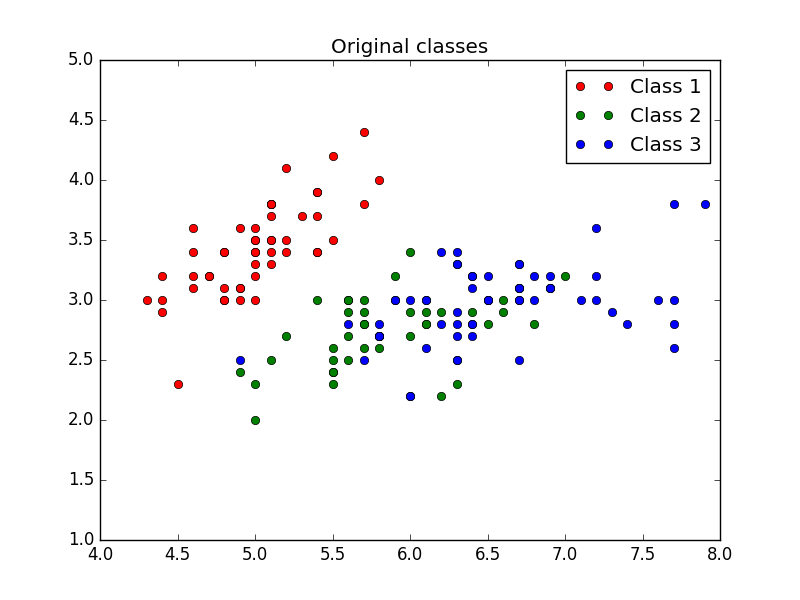
\includegraphics[width=0.7\linewidth]{./img/32b1.png}
	
	\centering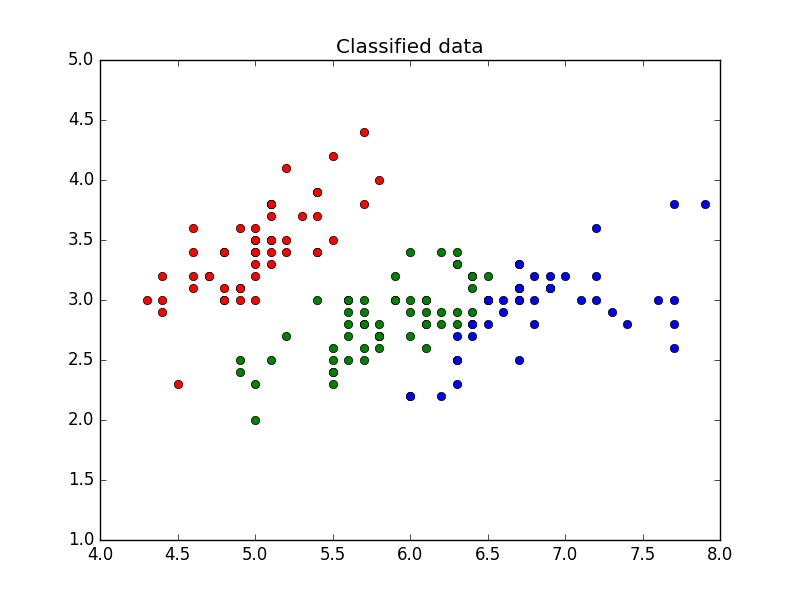
\includegraphics[width=0.7\linewidth]{./img/32b2.png}
	
	\lstinputlisting[language=Python, firstline=6, lastline=12]{../Code/32a.py}
	
\end{answer}
\end{question}

%----------------------------------------------

\end{questions}
